\begin{figure}[tb]
       \begin{center}
		   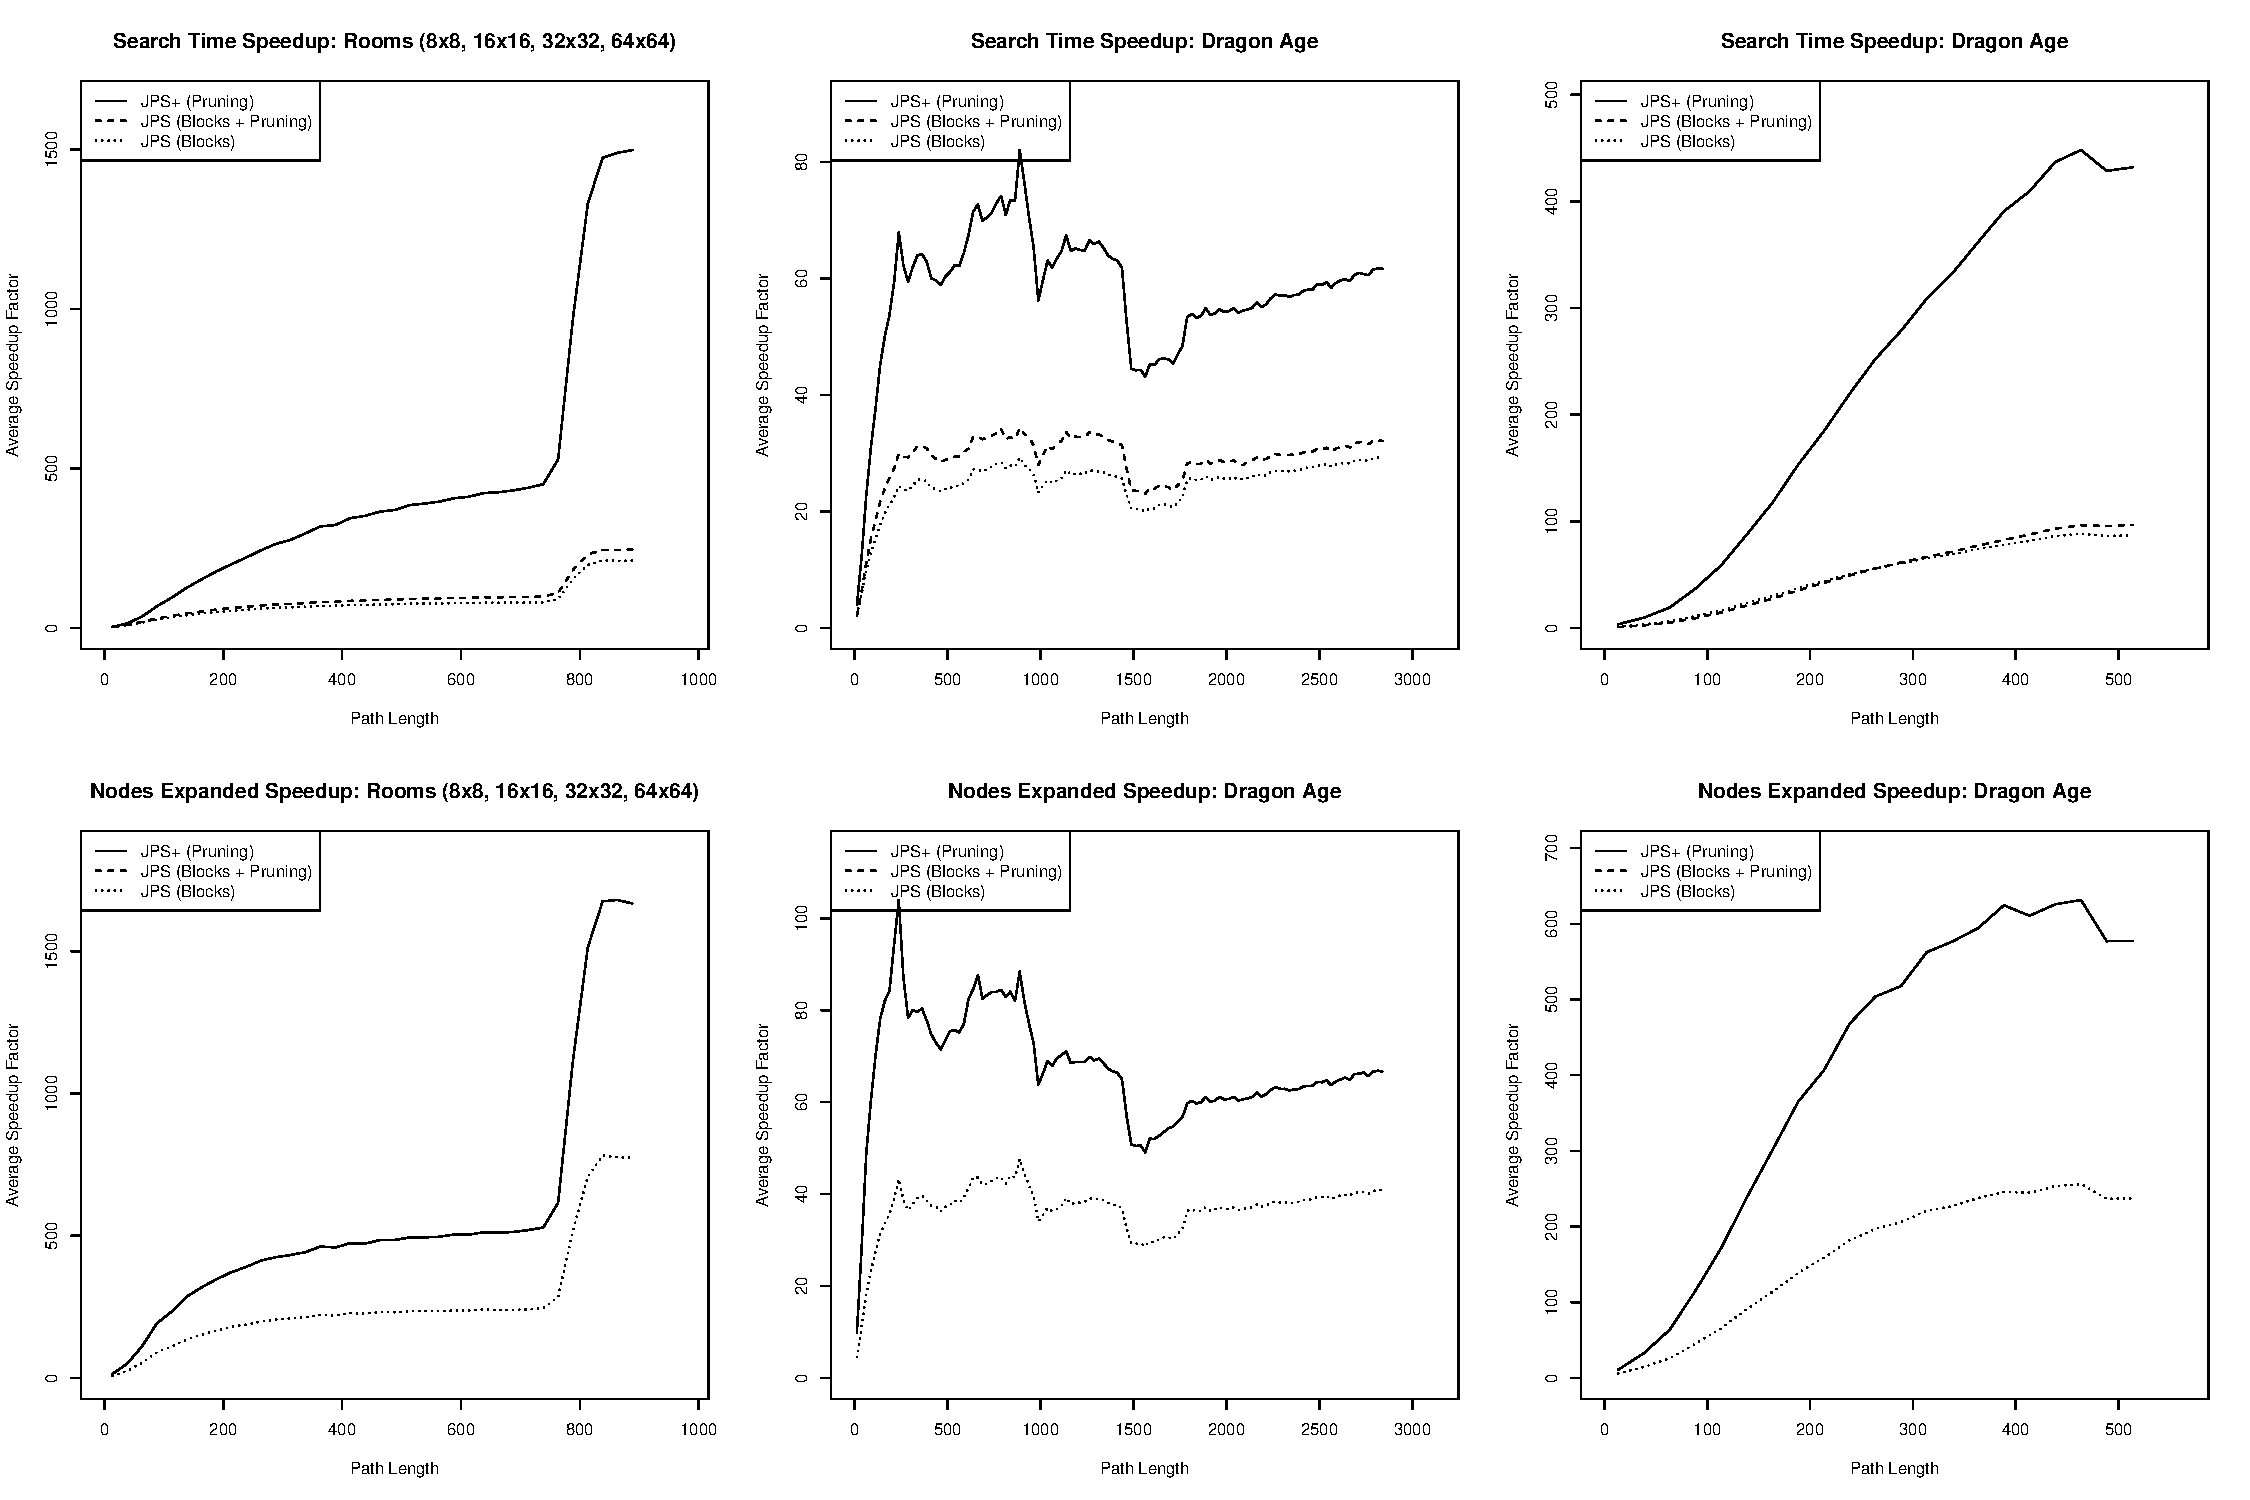
\includegraphics[width=0.95\columnwidth, trim = 0mm 0mm 0mm 0mm]
			{diagrams/speedup.pdf}
       \end{center}
\caption{Average search time speedup and average node expansion speedup for our three benchmark problem sets. In each case we measure relative improvement vs. A* 
across a range of instances. Higher is always better. NB: Algorithms JPS (B+P) and JPS+ (P) always expand the same number of nodes. }
\label{fig::node_speedup}
\end{figure}

\section{Results}
\label{sec::results}

We analyse the impact on search performance for each of our three optimisation techniques:
block-based jumping, denoted by JPS (B); improved pruning rules, denoted by JPS (P) and 
pre-processed jump point database, denoted by JPS+.
Where applicable we also give results for various combinations of these techiques. These 
variants follow a similar naming pattern.

We begin with Figure~\ref{fig::speedup} which performance results on each of our three
benchmarks in terms of average search time and average nodes expanded. We measure performance
in terms of relative improvement compared with A*. A speedup value of 2 for example indicates 
a two-fold improvement. Under this scheme, higher values are always better.

\begin{figure}[tb]
       \begin{center}
		   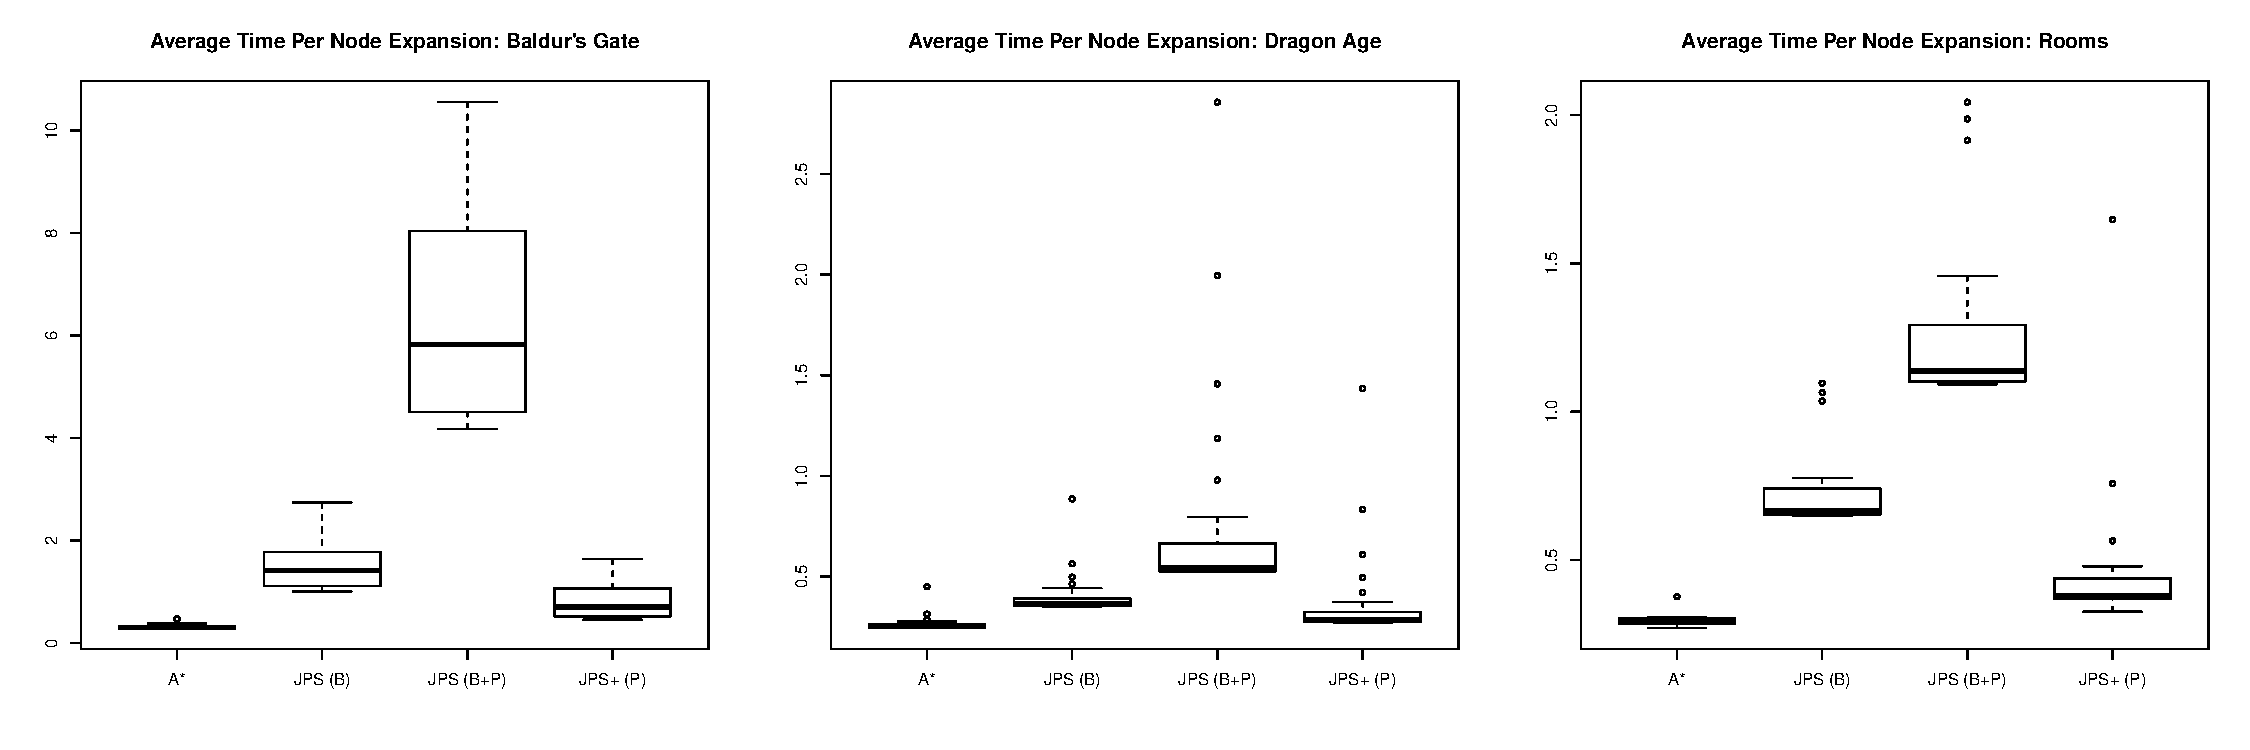
\includegraphics[width=0.95\columnwidth, trim = 0mm 0mm 0mm 0mm]
			{diagrams/avg_time_per_node.pdf}
       \end{center}
\caption{Average time, in micro-seconds, to expand a single node. We give a distribution of values showing the performance of each algorithm
on each of our three benchmarks. NB: the range of values along the y-axis differ in each case.}
\label{fig::node_speedup}
\end{figure}

Next, we turn our attention to Figure~\ref{fig::expansion_time} which measures
performance in terms of the average time, in mico-seconds, needed to expand a single node.
It is interesting to observe that in each case the lowest values are attributed to A*. 
JPS (B) and JPS (B+P), which both perform online symmetry breaking, always record
the highest values. These figures are in stark contrast with Figure~\ref{fig::speedup} where
the opposite is true. These results indicate that although eliminating path symmetries can have
a dramatic positive effect on overall search time, individual node expansions can incur a 
significant overhead. Thus, if the start and goal are very close, it is sometimes possible that
A* will be faster than Jump Point Search. The same is also true if JPS must explore very large
empty areas which contain nodes that appear promising but e.g. eventually lead to a dead-end.

